\documentclass[10pt]{article} \usepackage[a4paper]{geometry}
\geometry{verbose,tmargin=25mm,bmargin=25mm,lmargin=40mm,rmargin=10mm}
\usepackage{color}
\usepackage{array}
\usepackage{multirow}
\usepackage{amsmath}
\usepackage{setspace}
\usepackage{graphicx}
\usepackage{subfig}
\usepackage{siunitx}
\usepackage{amsmath}
\doublespacing
\usepackage[pdfusetitle,bookmarks=true,pdfborder={0 0
1},colorlinks=true]{hyperref}
\hypersetup{linkcolor=black,citecolor=black,filecolor=black,urlcolor=black}

\DeclareSIUnit\inch{in}

\usepackage{acronym}

\acrodef{GPU}{Graphics Processing Unit}
\acrodef{CPU}{Central Processing Unit}
\acrodef{SIMD}{Single Instruction Mulitple Data}
\acrodef{GPR}{General Purpose Register}
\acrodef{DLL}{Dynamic Link Library}
\acrodef{CRT}{C Runtime Library}
\acrodef{CSV}{Comma Seperated Variable}

\begin{document}

\begin{titlepage}
  \setlength{\parindent}{0cm}

  
\includegraphics[width=200px]{Images/uob-logo-black-transparent}

  \Large
  Faculty of Engineering and Design

  \vspace{80pt}

  \LARGE
  Final Year MEng Project \\
  Project Report

  \vspace{80pt}
  \textbf{Robot Football - High Level Control and Strategy Implementation}

  \vspace{10pt}
  \emph{Anthony Richards} \\
  \emph{\today}

  \vspace{80pt}
  Supervisor: \emph{Dr.~Pejman Iravani}

  \vspace{10pt}
  Assessor: \emph{TBD}
\end{titlepage}

\pagenumbering{roman}

\begin{abstract}
\acresetall
TODO : Abstract
\end{abstract}

\tableofcontents

\acresetall



\cleardoublepage

\pagenumbering{arabic}

\section{Introduction}

Discuss: 
Initial plan to use route planning and prediction
Discovery that route planning would have to be done far to regularly to be
feasible
Discovery that route planning would be vvv CPU intensive
Decision to explore artificial potential field force navigation

\section{Literature Review}

\section{Computational Methods}

\subsection{Motion Control}

\subsubsection{Simulator Characteristics}

No documentation has been provided for the simulation, and so all of the
characteristics of the system need to be determined before a working system can
be produced.

There are two methods of timing that the system could use:
\begin{itemize}
 \item Fixed time-step - Every simulator cycle is assumed to be a constant
 length
 \item Variable time-step - The time-step length is proportional to the
 wall-time elapsed since the last time-step.
\end{itemize}

The real-time length of each time-step was recorded over a period of period of
time.  If a fixed time-step is used, and the simulator is attempting to run in
real-time, the results should show most of the readings at this timestep level,
 with others longer but none singificantly shorter.  A free running real-time
 simulator would display a varying timestep depending on the length of the
 instructions to be executed each cycle, as well as any other activities
 currently taking place on the computer.  This, however, would not be a
 conclusive result, as fixed time-step simulator that isn't running in real-time
 would display similar results.

The distribution produced is shown in figure \ref{fig:timestepDistribution}.  As
 can be seen, the real time-step length varies from
 \SIrange{17.5}{26.0}{\milli\second}, with an approximate normal distribution
 around the mean of \SI{19.17}{\milli\second}.  As discussed previously, it is
 not possible to use this result to determine the simulator's timestep type.
 This could result could equally be a variable time-step length which is being
 effected by other operations on the computer, a real-time fixed time-step
 simulation that is suffering from clock jitter or a fixed time-step simulation
 not running in real-time.

\begin{figure}
 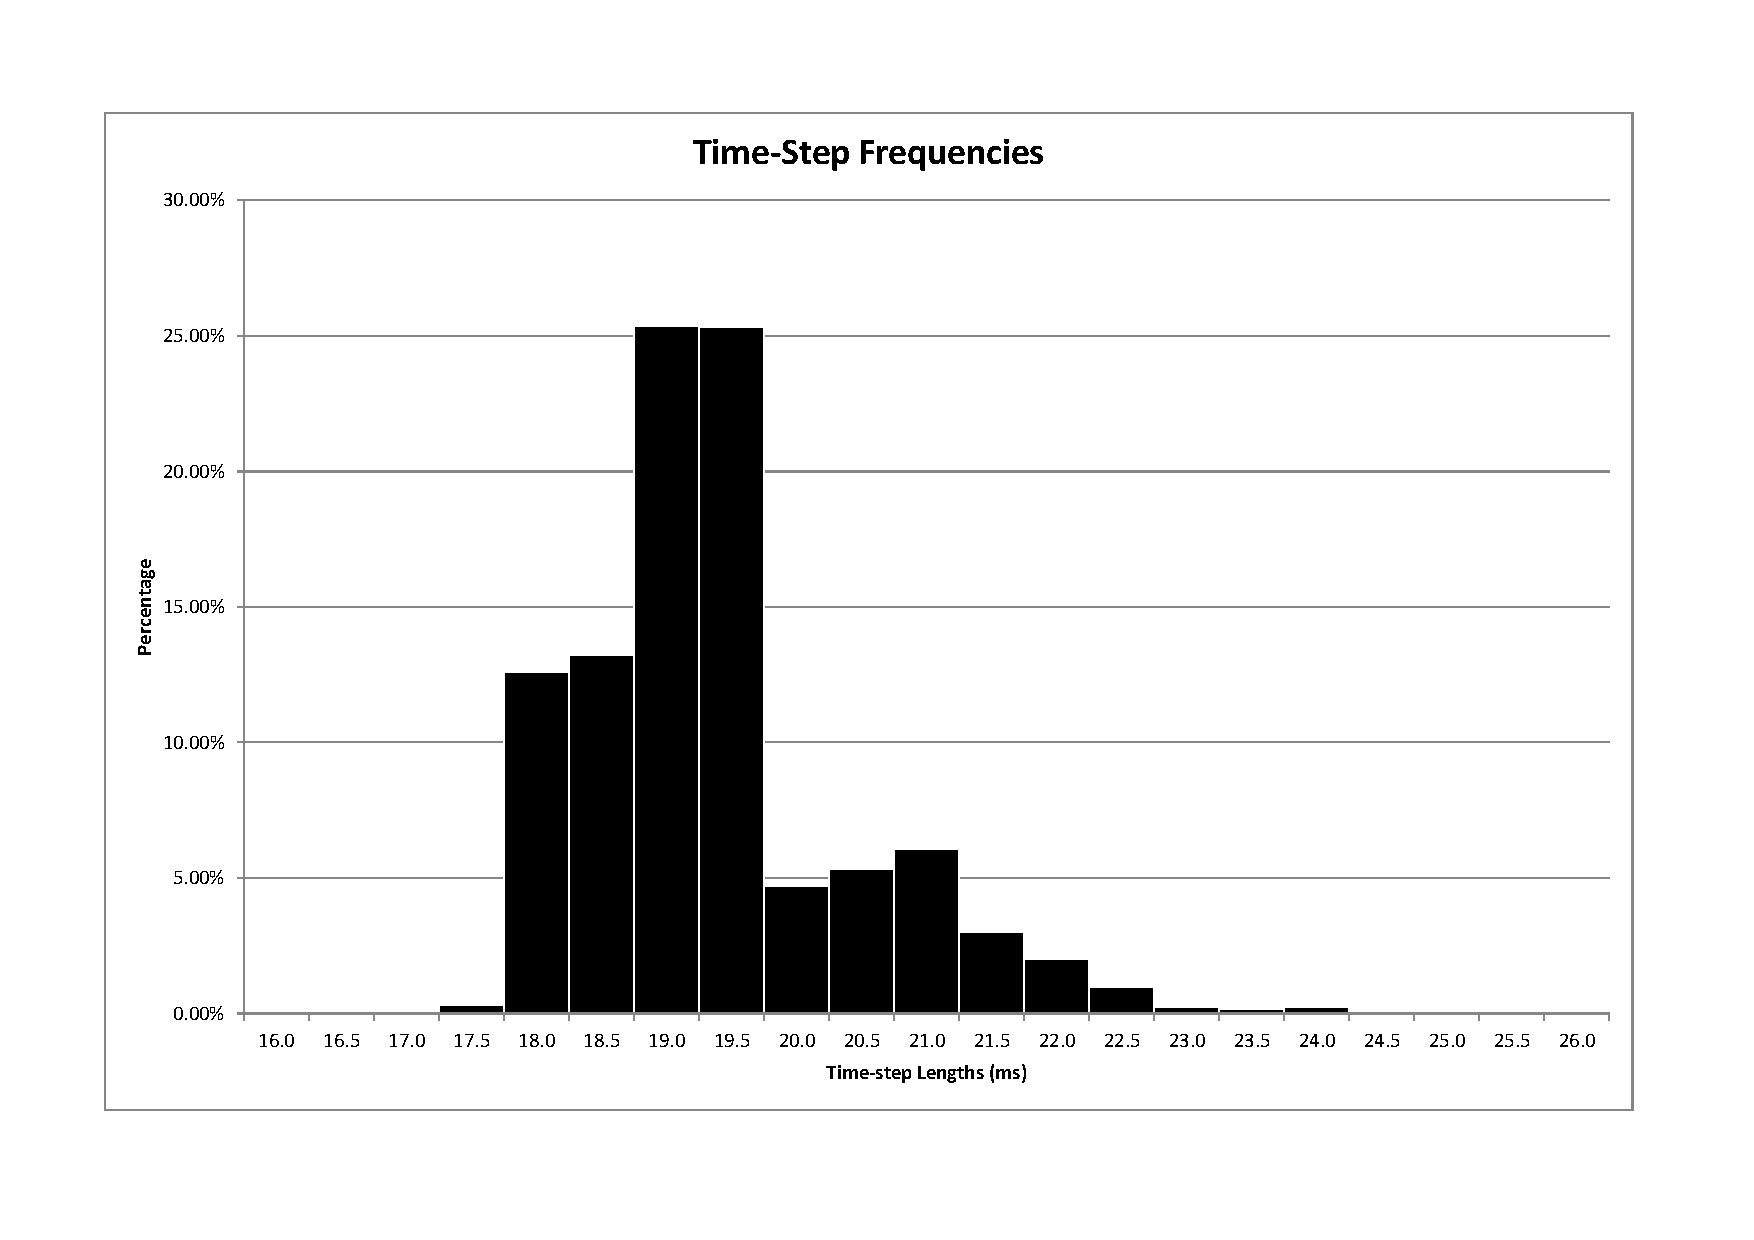
\includegraphics[width=\textwidth]{Images/time-step-length-distribution} \\
 Mean : \SI{19.17}{\milli\second} \\
 Standard Deviation : \SI{1.258}{\milli\second}

 \caption{Time-step Frequency Distribution}
 \label{fig:timestepDistribution}
\end{figure}

An initial run was set up to examine the behaviour of the system over time, and
is shown in figure \ref{fig:initialSpeedTestRun}.  The velocity of the system
(which is determined by dividing the distance travelled by the timestep) has
been calculated with both the measured timestep, as well as a fixed timestep of
\SI{20}{\milli\second} (chosen as a round number approximating the values
measured). The actual value of the fixed time-step is not a concern, as it will
only have a scaling effect on the velocity, which can be accounted for later.

The calculation with a variable timestep (figure
\ref{fig:initialSpeedTestRunVariable}) displays a significant oscilation of the
velocity around the expected behaviour.  In contrast, the fixed time-step values
almost exactly matches the expected behaviour (figure
\ref{fig:initialSpeedTestRunFixed}).  While it is possible that the simulator
could be emulating a non-steady output velocity from the motors, it is expected
that this would display in both graphs.  This makes it very likely that the
time-step used by the simulator has a fixed length.

The anomoly displayed at approximatly \SI{0.6}{\second} on figure
\ref{fig:initialSpeedTestRunFixed} is also seen in a large number of the other
recordings made of this particular scenario.  This is not due to an overly long
simulator cycle length, as this would be hidden by the fixed time-step length.
The fact that it is present shows that there were one or more simulator cycles
where the system was not updated.  This suggests that it is due to a bug in the
simulator, and any controller will need to be able to handle this sort of error
with minimum disruption.

Next, it was necessary 

\begin{figure}
 \centering
 \subfloat[Variable Time-step Length Initial Run
 Velocity]{\label{fig:initialSpeedTestRunVariable}
 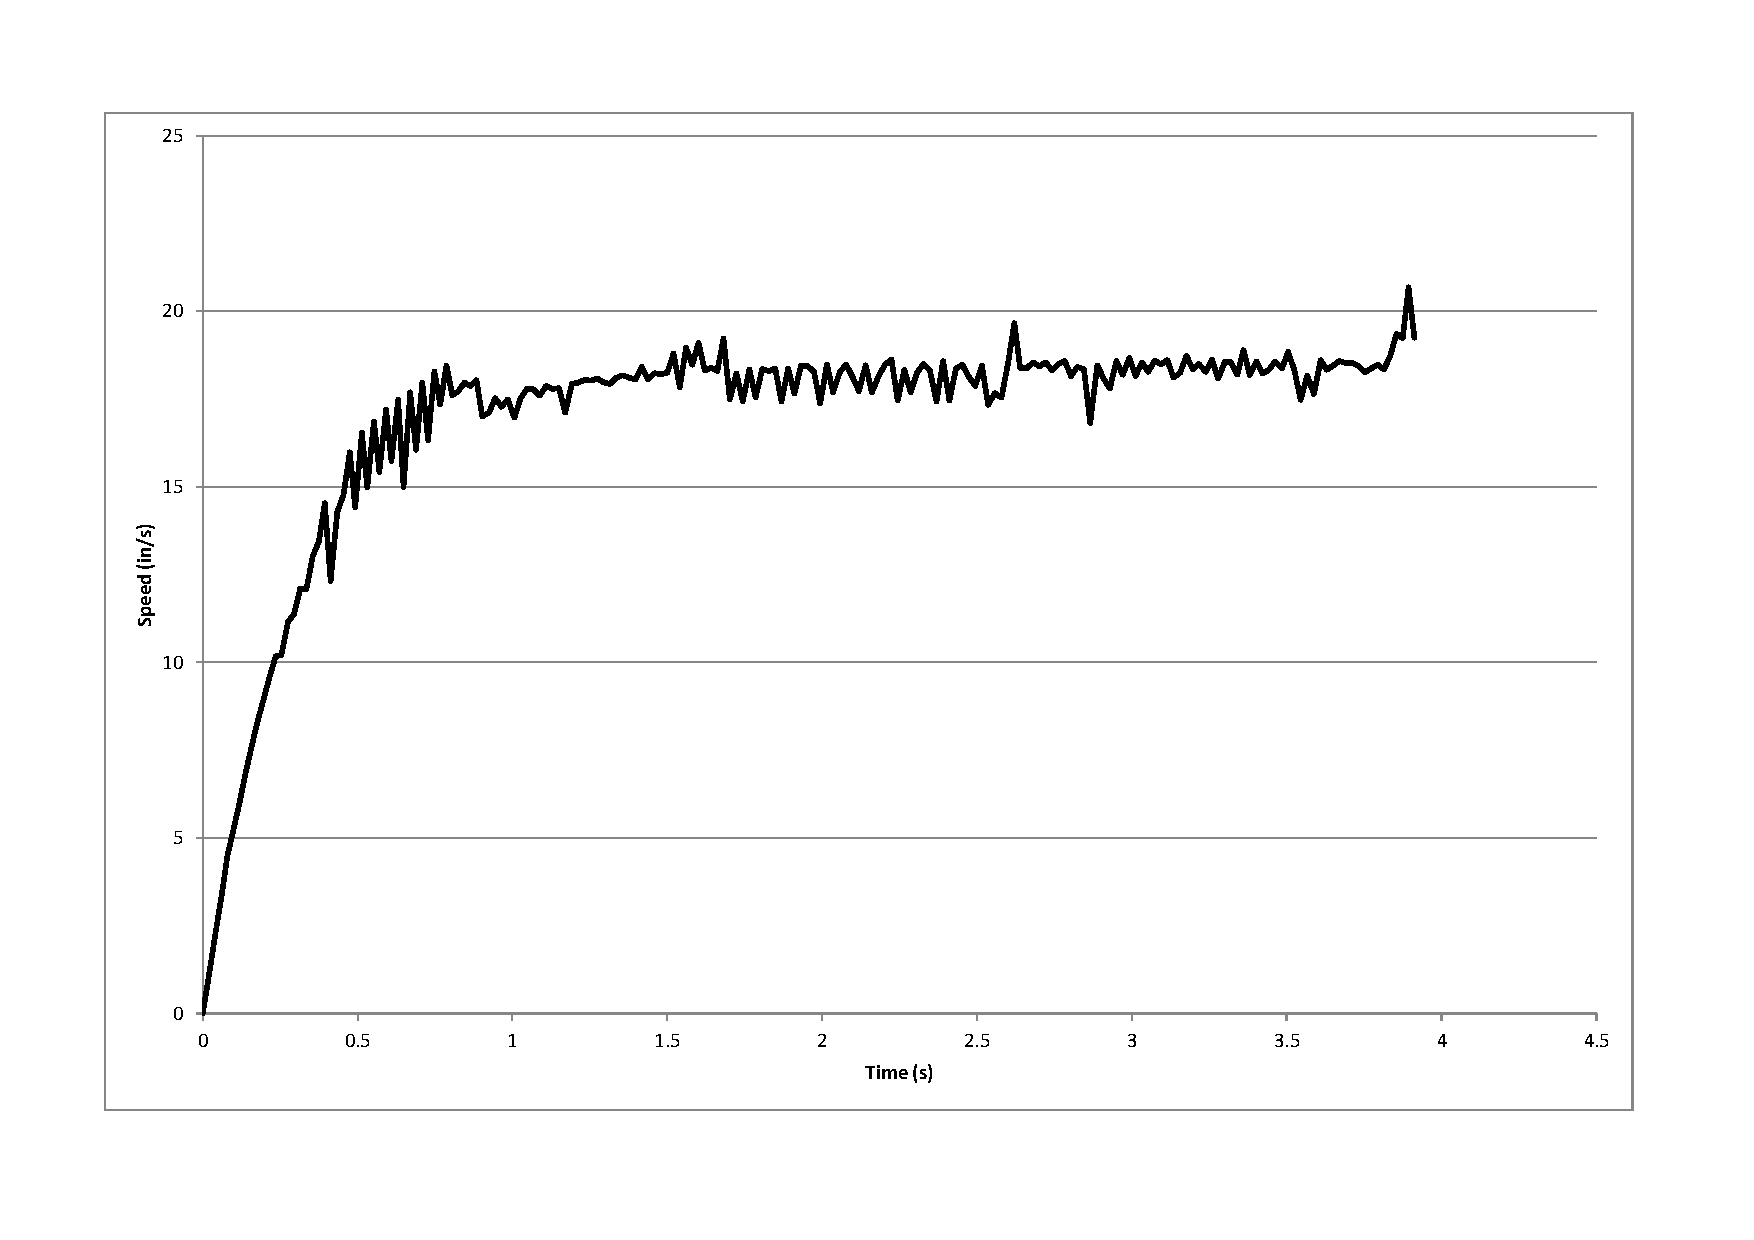
\includegraphics[width=0.8\textwidth]{Images/variable-time-step-initial-run}}
 \\
 \subfloat[Fixed Time-step Length Initial Run
 Velocity]{\label{fig:initialSpeedTestRunFixed}
 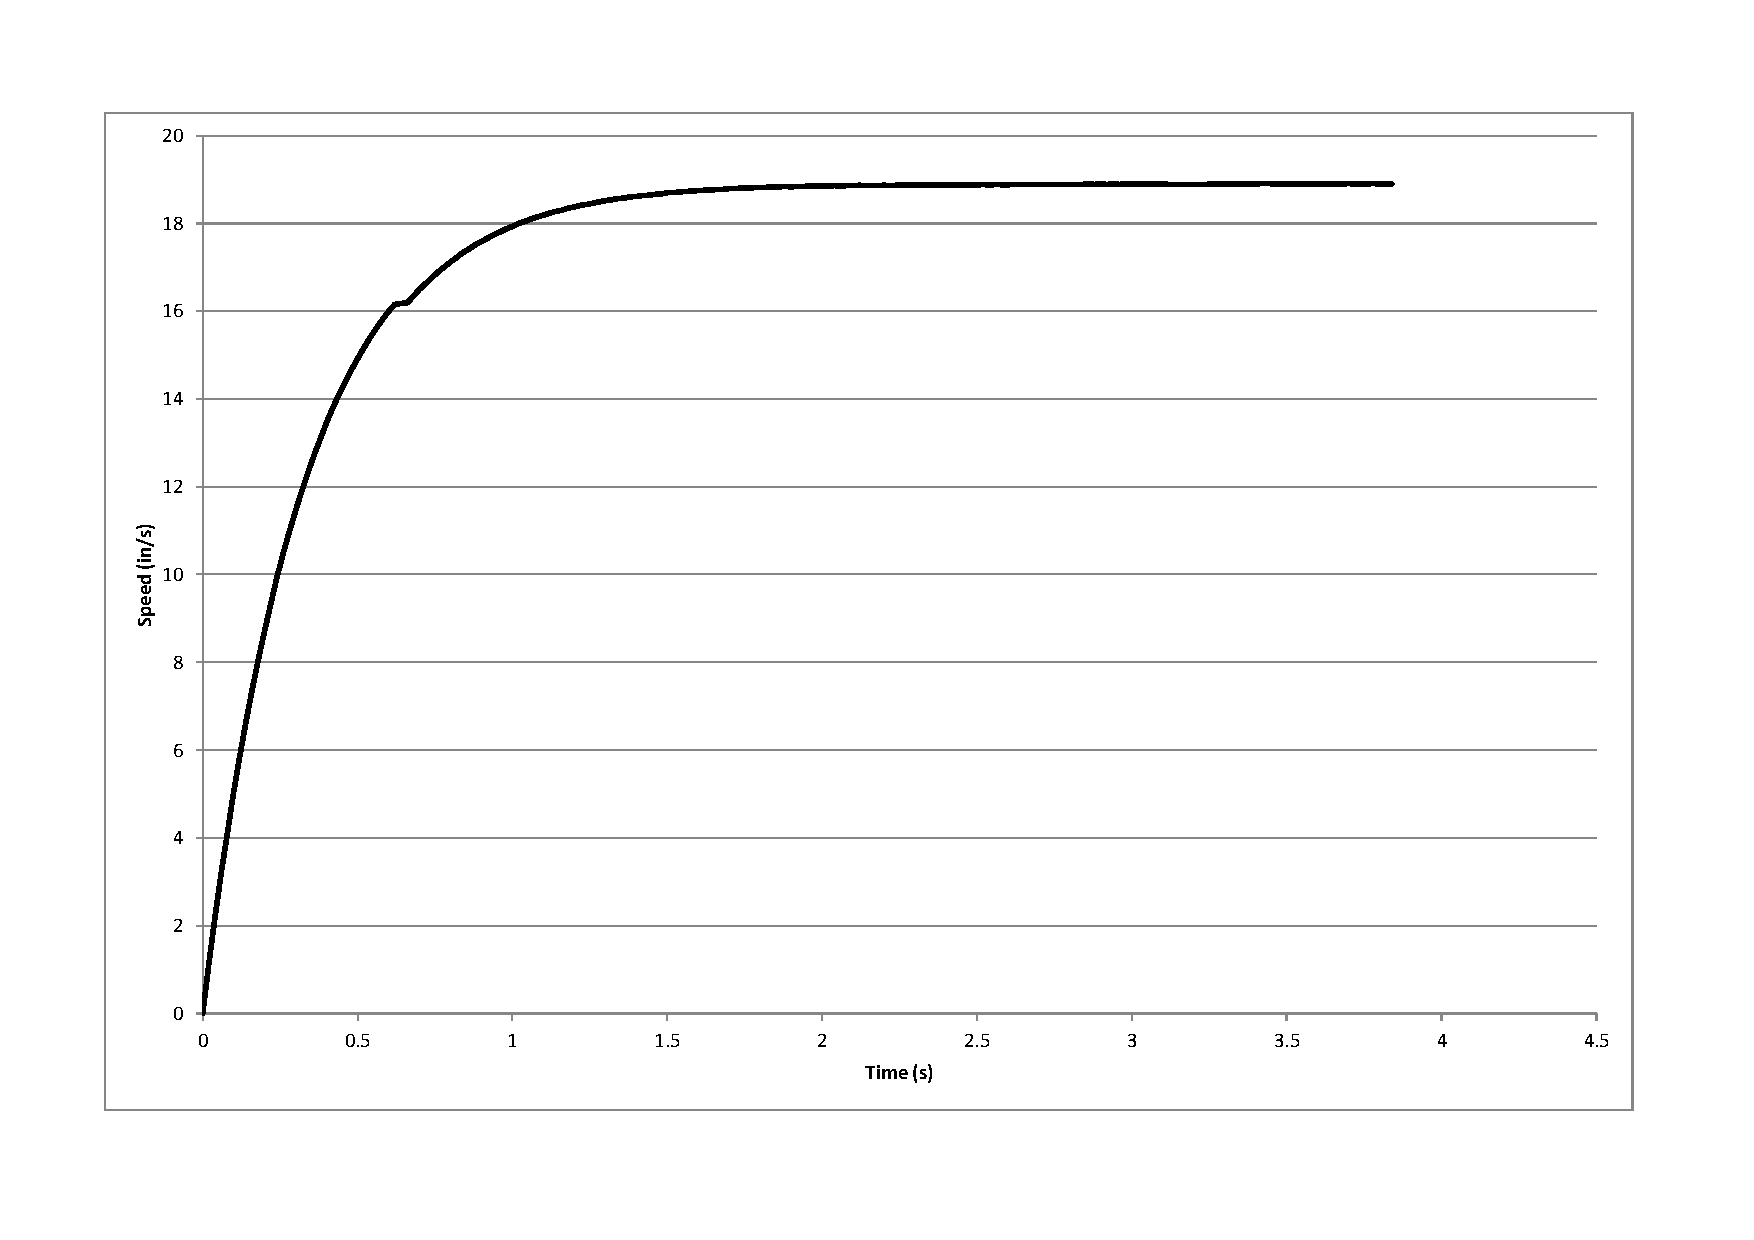
\includegraphics[width=0.8\textwidth]{Images/fixed-time-step-initial-run}}
 \caption{Initial Run Velocities}
 \label{fig:initialSpeedTestRun}
\end{figure}

Finally, it was observed that the simulation pauses when the simulator loses the
user focus.  It then resumes without anomaly when the simulator regains the
focus.  As the simulator does not inform this strategies of this, and does not
provide the strategies with any timing data, it is unreasonable to believe that
real-time values are in use.  Were they used, the strategies would experience
control issues caused by the anomalously long time-step if the simulator lost
the focus (and so was suspended) for a significant period of time.  For this
reason, it was assumed that a fixed time-step length was in use, and the length
chosen is \SI{20}{\milli\second}.

As well as the timing details, the coordinate system in use by the system needed
to be determined.  The conventional coordinate system used by computer programs
is often the same as the system used by the computer graphics systems.  This
defines $\left(0,0\right)$ as the top-left corner, with positive $x$ pointing to
the right of the screen and positive $y$ pointing down the screen.  The
trigonometric functions provided by the \ac{CRT} operate using radians, and the
specification for the playing field is provided in metric units.  It was
initially assumed that the simulator would follow these conventions, but this
was quickly disproved.

Examination of the header files provided to support the simulator revealed that
the basic constants describing the field were defined in inches. The constants
provided also defined the bottom of the field (as shown on the screen) at a
lower coordinate than the top.  These two facts define the position coordinate
frame.

The units of rotation were not defined in the header files, and so had to be
found by experimentation.  One of the robots was controlled to spin on the spot
by driving the motors in opposite directions.  The reported angle of rotation
was then monitored using a debugger as each cycle passed.  This showed that the
angle reported varied between from \numrange{+180}{-180}.  This infers that the
coordinate system is using degrees to represent angles, and means that
conversion will need to be made to allow the \ac{CRT} trigonometric functions.

\subsubsection{Uncontrolled Behaviour}

The model used for the robots in the simulator is also not documented. It is
therefore assumed that the robot's motion is modelled on that produced by an
electric motor. The basic behaviour of the system should be described by the
transfer function in equation \ref{eq:basicMotorModel} \cite{basicControlNotes}.

\begin{equation}
 \label{eq:basicMotorModel}
 G\left(s\right) = A \cdot \frac{1}{s+B}
\end{equation}

In order to determine the values of the constants $A$ and $B$, a simple strategy
was set up that fed one of the robots a fixed control signal.  This caused it to
accelerate in a straight line until it reached a constant speed.  The position
at each timestep was recorded, to allow the velocity and acceleration to be
calculated.  This was repeated with a number of different input signals, until
the robot could no longer achieve a stead-state speed without colliding with a
wall.

If the model is correct, the steady-state velocity should be directly
proportional to the input velocity.  The steady-state velocity was calculated by
averaging the final ten samples of each simulation, and is plotted against input
signal in figure \ref{fig:inputOutputVelocityGraph}.  A line of best fit has
been plotted to demonstrates the linear relationship between input and output.

It is interesting to note that the best fit ($R^2 = 1$) is achieved if the
constraint that zero input produces zero output is removed.  This infers that
there is a systematic error that is being introduced by the simulation.  This
will be disregarded in this case, as the error is small
(\SI{-0.3405}{\inch\per\second}) and so should have minimal effect on the
behaviour of the controller.

Given that the the output velocity is 0.7564 times the input velocity, it was
next necessary to find the theoretical maximum velocity of the robot.  This was
first achieved by passing the simulator a very large number to determine it's
response.  It was quickly noted that the simulator caps the input value at 125.
This gives a theoretical maximum velocity of \SI{94.55}{\inch\per\second}.   It
was noted at during this experimentation that the robot could not reach it's
theoretical full speed without colliding with a ball.

In order to determine the equation controlling the system, the velocity data was
first normalised by dividing it by the input signal.  This allows the various
volecity profiles recorded to be compared.  The systematic error observed will
cause the data to become slightly distorted, but as previously mentioned, it is
believed the effect will be small.  The MATLAB Curve Fitting Toolbox was then
used to fit the data to a curve.

The best fit achieved is shown in figure \ref{fig:bestFit}.  This is fitting the
data to an equation of the form $y = a \cdot e^{bx} - c \cdot e^{dx} $.  The
function was expected to be of the form $y = a(1-b \cdot e^{cx})$, as this is
what is the form of the time-domain response of the theoretical model in
equation \ref{eq:basicMotorModel} to a step-input.

It was noted that the $b$ term is very small, and the $a$ and $c$ terms are
approximatly the same.  Therefore, it was expected that the model could be
approximated with an equation of the latter form.  This is illustrated in figure
\ref{fig:approximateFit}, which demonstrates an acceptable fit to the majority
of the data.  It is noted that the steady-state velocity implied by this model
is different to that calculated earlier.  However, it is anticipated that the
robot will rarely be moving at a constant velocity for long, and this model
gives a good approximation of the dynamic behaviour shown by the system.

It was noted that some of the data in the plot appears to be shifted along in
the time-axis, and which is likely interfering with the line fitting process.
This was determined to be due to an error in the original data, where the time
had not been reset to zero at an appropriate point on one of the test runs.
When the data was shifted back into a more expected location, the approximate
fit was improved (shown in figure \ref{fig:approximateFitTimeShiftRemoved}).

Using this information, the system can be modelled with equation
\ref{eq:finalMotorModel}.  This was then used to design the control systems
required.

\begin{equation}
 \label{eq:finalMotorModel}
 G\left(s\right) = \frac{2.12778}{s+2.863}
\end{equation}

\begin{figure}
 \centering
 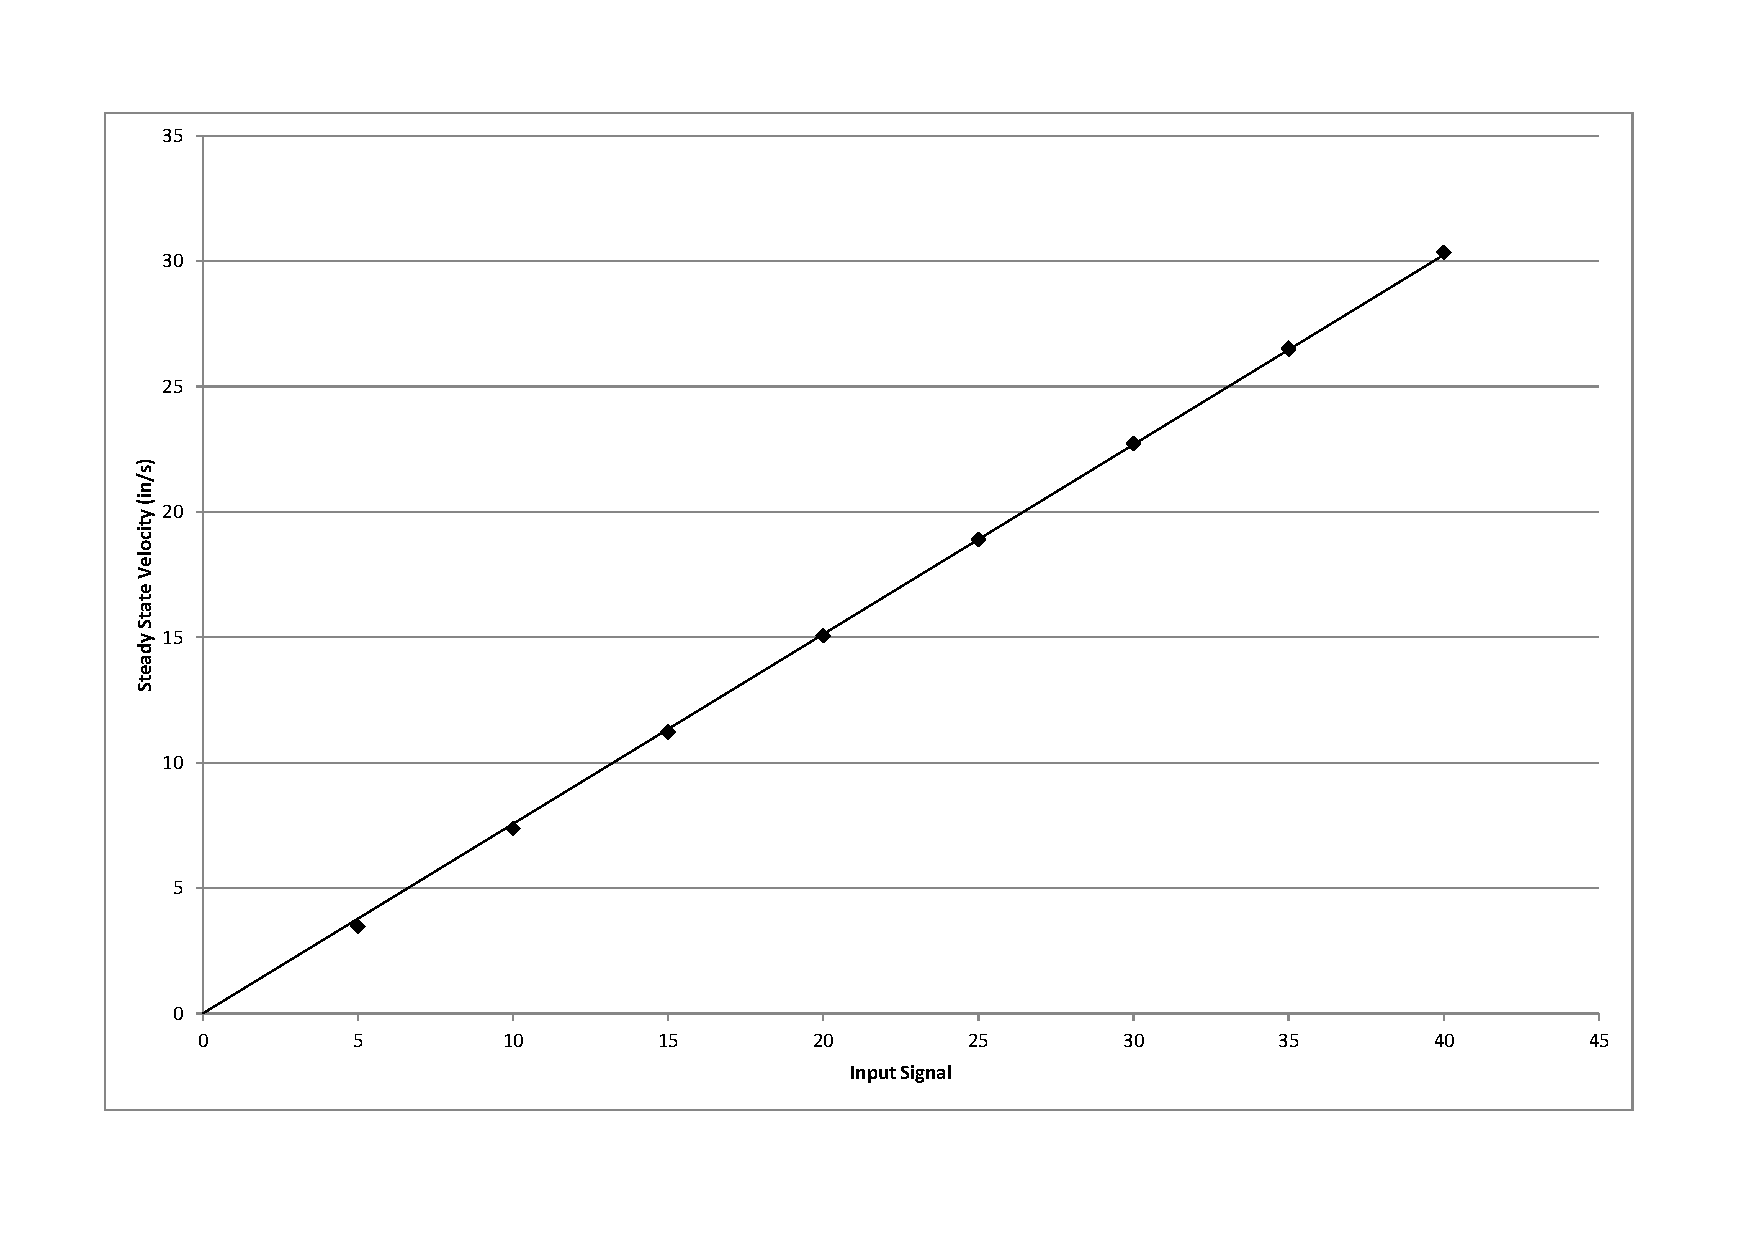
\includegraphics[width=0.8\textwidth]{Images/input-signal-vs-output-speed}
 \caption{Input Control Signal vs Output Velocity}
 \label{fig:inputOutputVelocityGraph}

 Line of best fit: $y=0.7564x$ \\
 Quality of fit: $R^2 = 0.9998$
\end{figure}

\begin{figure}
 \centering
 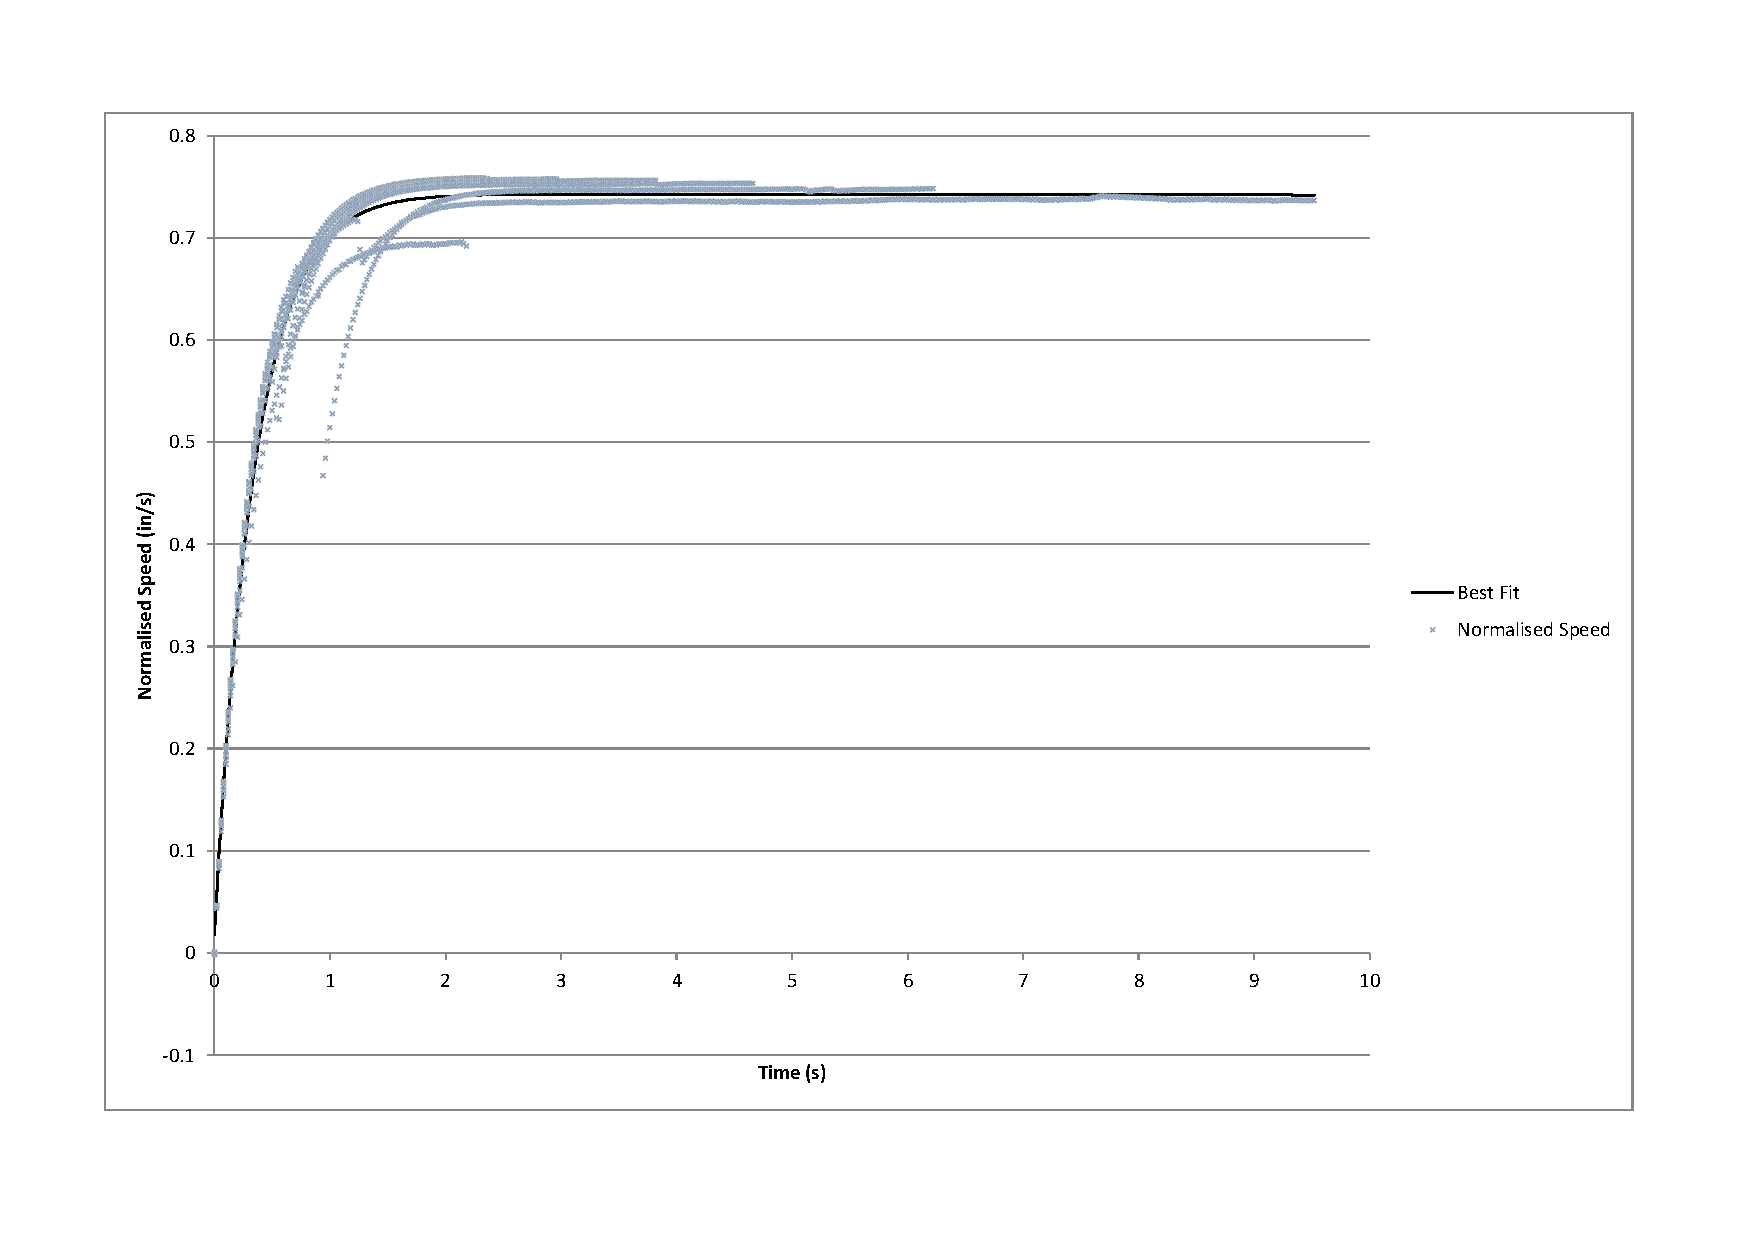
\includegraphics[width=0.8\textwidth]{Images/best-fit-model}
 \caption{Curve Fitting Toolbox Best Fit}
 \label{fig:bestFit}

 Line of best fit : $y=0.7432 e^{-0.0001886x}-0.7248 e^{-2.863x}$ \\
 Quality of fit : $R^2 = 0.976$
\end{figure}

\begin{figure}
 \centering
 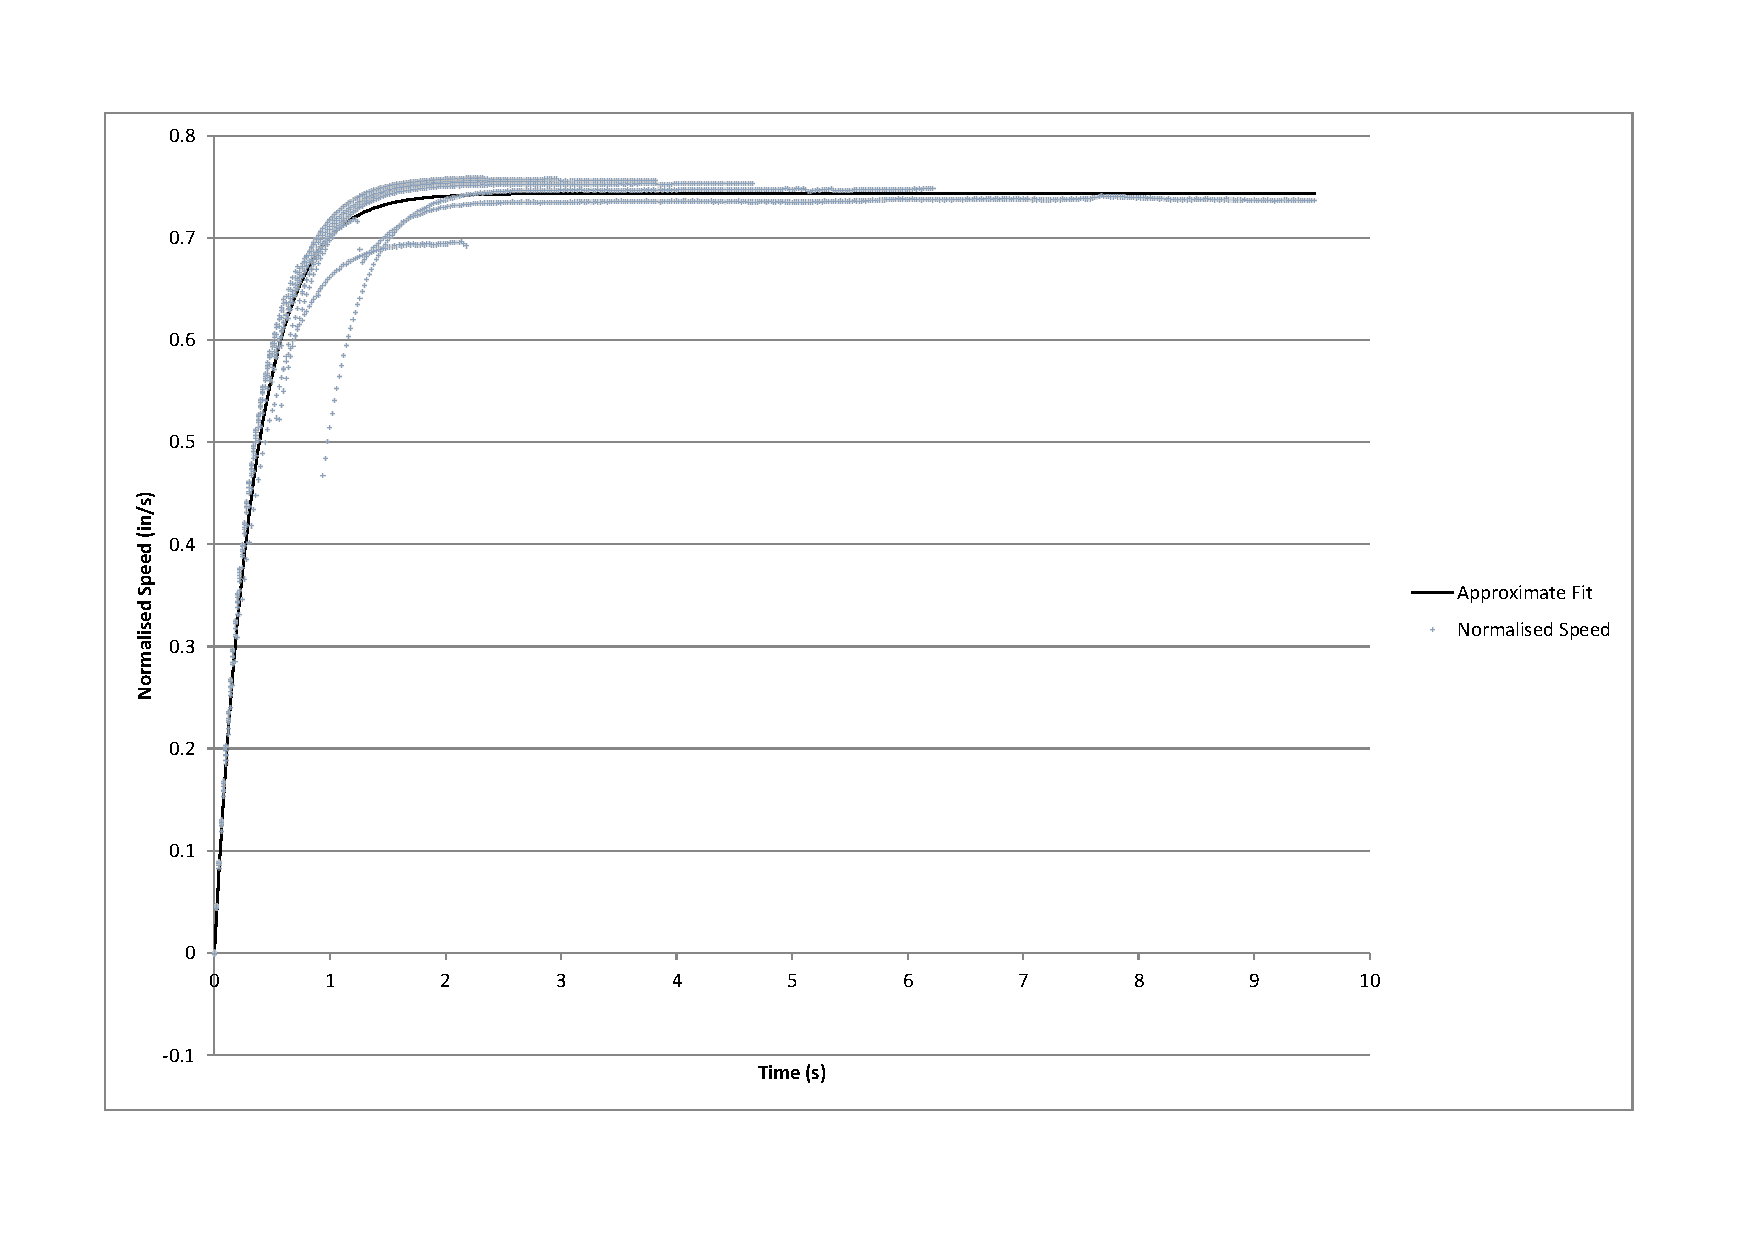
\includegraphics[width=0.8\textwidth]{Images/approximate-fit-model}
 \caption{Approximated Curve Fit}
 \label{fig:approximateFit}

 Line of best fit : $y=0.7432 \left(1-e^{-2.863x}\right)$
\end{figure}

\begin{figure}
 \centering
 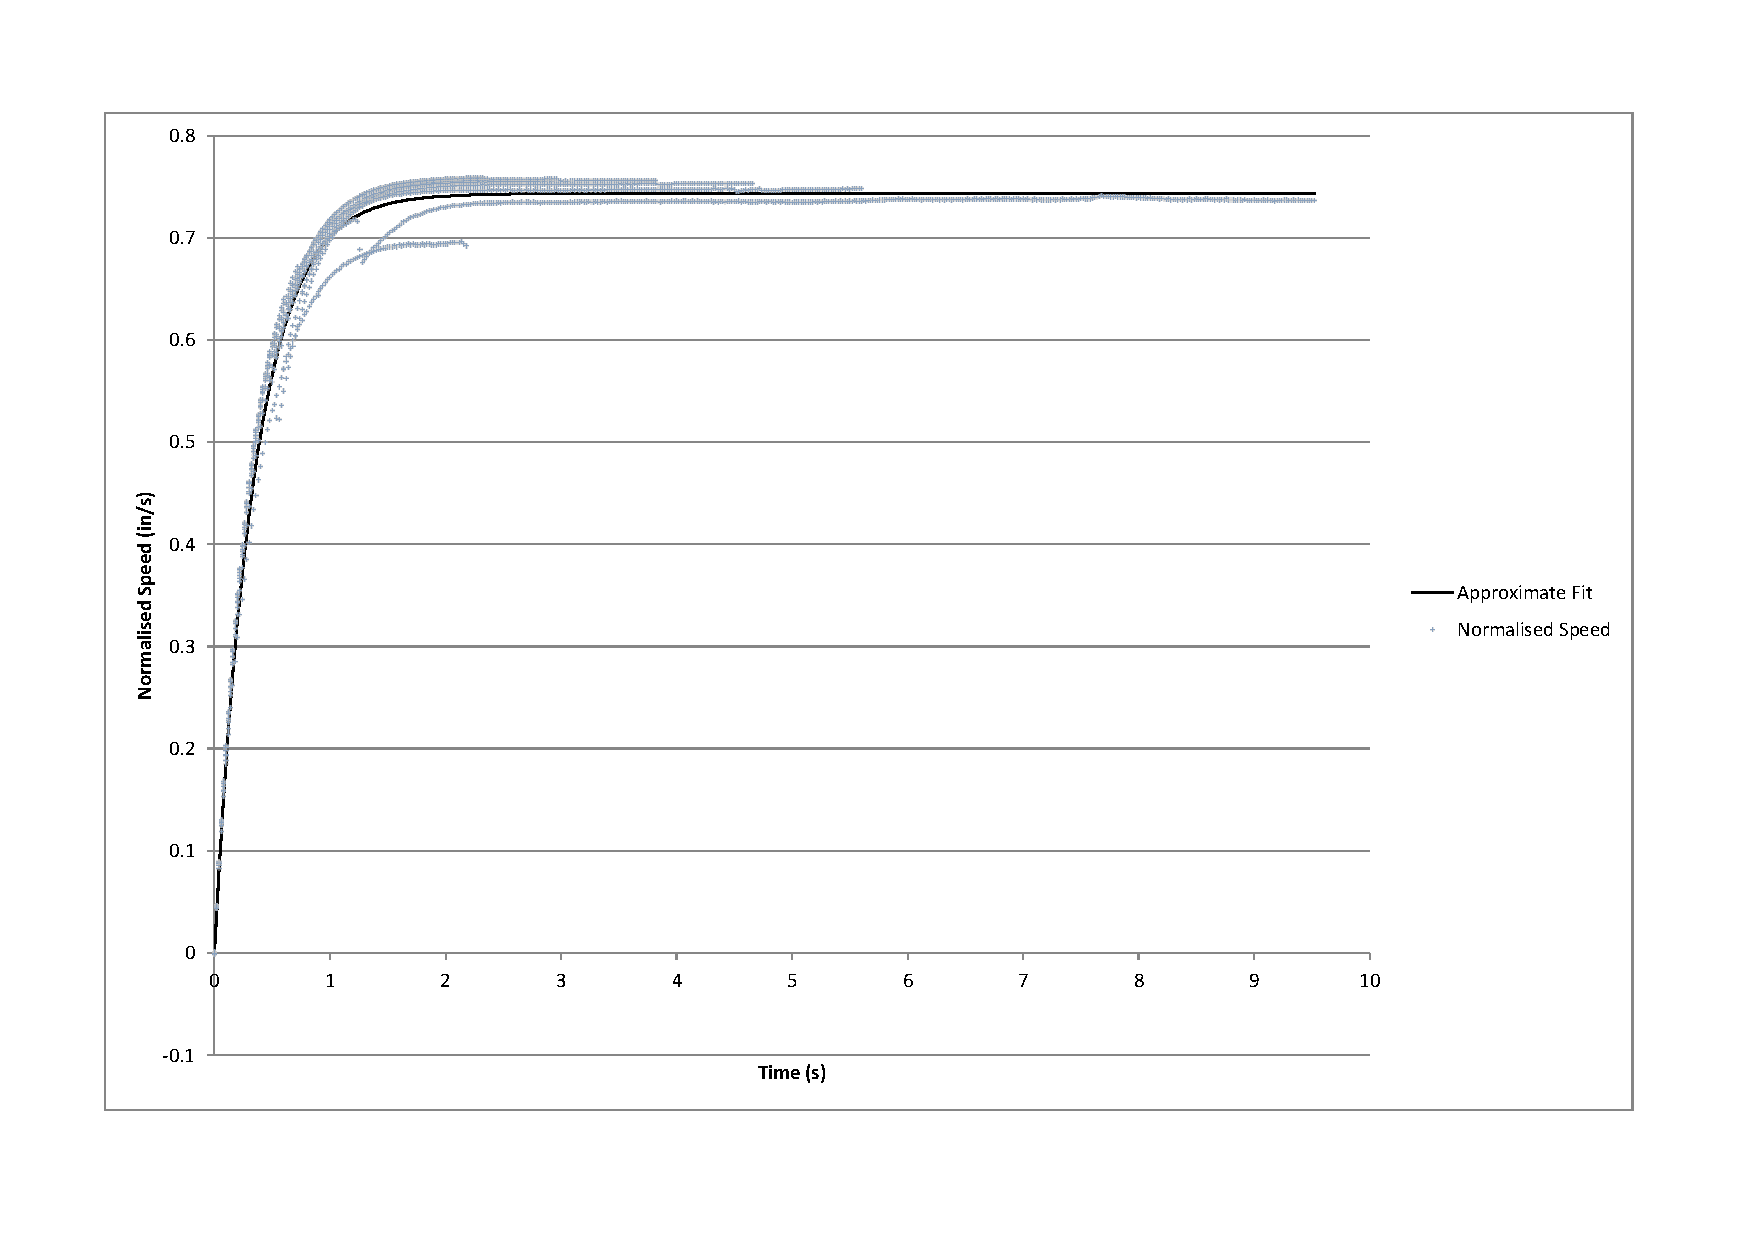
\includegraphics[width=0.8\textwidth]{Images/approximate-fit-model-time-shift}
 \caption{Approximated Curve Fit with Corrected Data}
 \label{fig:approximateFitTimeShiftRemoved}

 Line of best fit : $y=0.7432 \left(1-e^{-2.863x}\right)$
\end{figure}

\subsubsection{Controllers}

In order to allow the control of position or velocity desired, the motion
control was implemented using two layers of control.  The first layer controls
the velocity of the robot, while the second layer manipulates the first to
control position.

Both layers are simple proportional controllers, with the velocity control
receiving velocity feedback and the position control receiving position
feedback.  The overall control design is shown in figure
\ref{fig:overalController}.

The gains were tuned using the MATLAB controller design tools.  The velocity
controller were handled first, to ensure that it would stand alone, and then
motion controller was tuned to adequatly control the resulting velocity.  The
gains calculated were then transferred to the C++ classes VelocityController and
MotionController to be tested.

Unfortunatly, when the code was tested, it was found that the system was highly
unstable, and the specific reasons could not be isolated.  As the aim of the
project was to investigate the high-level control of the robot, rather than the
low-level motor control, the problem was not closely examined.  Instead a set of
gains were produced by a trial-and-error method, which produced a sub-optimal
but stable system.

The control of the angle of motion was achieved by noting the similarity between
the robot footballers and the Mouse robot used in the second year project
\cite{mouseProjectReport}.  The direction of motion was changed by altering the
relative velocities of the individual wheels, which causes the robot to move
through an arc.  Proportional control was again used for this purpose, with the
velocity different proportional to the angular error.

It is recognised that the controllers in use are likely not the optimal designs
that could be used for the system.  While this will have an effect on the
performance of the robot (and so the range of motions that can be performed), it
was decided that investigating the higher level control was more important for
this specific work.  The effect of a better control system can then be
investigated in the future.

\subsection{Potential Field Force Navigation\label{sub:Potential-Field-Force}}

With this technique, a potential field is used to create a force that guides
each robot around the field (as described in
\cite{intelligentAlgorithmPathPlanning}). The field is produced by taking a
collection of objects and projecting a field around them of a given shape. This
field can either add to or subtract from the total field potential surrounding
it. The total field can then be calculated with equation
\ref{eq:fieldSummation}.

\begin{equation}
P(x,y)=\sum_{i=0}^{N-1}p_{i}\left(x,y\right)\label{eq:fieldSummation}
\end{equation}

Where:

$P\left(x,y\right)$ is the total field potential at point $\left(x,y\right)$.

$p_{i}\left(x,y\right)$ is the potential produced by object $i$ at a point.

$N$ is the number of field producing objects.

The direction that the robot will move in is then determined by the gradient of
the field at the current point, such that the robot moves down the field
potential. The force vector (which controls the velocity of the robot) is given
by equation \ref{eq:forceSummation}.

\begin{equation}
\boldsymbol{F}(x,y)=-\left(\frac{{\partial P\left(x,y\right)}}{\partial x}+\frac{{\partial P\left(x,y\right)}}{\partial y}j\right)\label{eq:forceSummation}
\end{equation}

If the fields can be differentiated over the entire field, this can be
calculated as in equation \ref{eq:forceDifferentiation}.

\begin{equation}
\boldsymbol{F}(x,y)=-\left(\sum_{i=0}^{N-1}\frac{\partial p_{i}\left(x,y\right)}{\partial x}+\frac{\partial p_{i}\left(x,y\right)}{\partial y}j\right)
\label{eq:forceDifferentiation}
\end{equation}

However, if one or more of the fields cannot be differentiated, the force vector
must be calculated discretely. This is achieved using equation
\ref{eq:forceDifferentiationDiscrete}.

\begin{equation}
\boldsymbol{F}(x,y)=\left(P\left(x-1,y\right)-P\left(x+1,y\right)\right)+\left(P\left(x,y-1\right)-P\left(x,y+1\right)\right)j
\label{eq:forceDifferentiationDiscrete}
\end{equation}

The negative gradient is used to ensure the robot moves towards lower field
potentials. The technique would work equally well if it was attracted to higher
field potentials, provided all the equations were suitably inverted.

For the initial control technique, the velocity of the robot is proportional to
the force vector. Other techniques are discussed by
\cite{intelligentAlgorithmPathPlanning}, but will be experimented on later.

Navigation of the game field can now be achieved by manipulating the attractive
and repulsive fields to guide the robot to a target. Computational power
allowing, each robot would have a separate field that guides it based on the
goals specific to its role.

\subsection{Potential Field Shapes}

Attractive fields are used to designate areas which the robot should heading
for. In order to ensure that the robot always moves towards them, it is
important that their effect is felt across the entire field. However, they must
not be so strong that they overwhelm the short distance effects of the repulsive
fields.

Repulsive fields are used to alter the route of the robot when moving towards
these targets. For example, such fields are used to get the robot to avoid
collisions, as well as to control where the robot intercepts the ball. These
fields typically only act over a short distance, as they should only have an
effect when they are required. They need to be strong enough to overwhelm the
attractive fields at short range.

The field shapes experimented with are described in the following sections, and
a selection of them were integrated into the final strategy, in order to produce
the best combination for each scenario.

As the basic fields in use are axisymmetric in shape (or begin that way), the
fields are best described using polar coordinates. The coordinates are defined
as in figure \ref{fig:polarCoordinateFrame}, and are always centred on the field
producing object. This frame of reference can then be translated to the
Cartesian coordinates in use elsewhere to allow the total field at a point to be
calculated.

\subsubsection{Basic Attractive Field\label{sub:Basic-Attractive-Field}}

The field suggested by \cite{intelligentAlgorithmPathPlanning} for the
attractive point is described with equation \ref{eq:quadraticBallField}.

\begin{equation}
P(r,\theta)=\frac{1}{2}k_{attr}r^{2}\label{eq:quadraticBallField}
\end{equation}

Where $k_{attr}$ is the attractive weight assigned to the ball.

This produces an attractive force that is linearly proportional to the distance
to the object (in this case the ball). This is a very useful field for a route
finder (as described in the paper), where it is desirable for the the robot to
stop when it reaches the destination, and so it needs to slow down as it
approaches the target. However, in this application it is more useful for the
robot to make a rapid approach and not slow down after arrival. This is because
the ball is not held to the robot in any way, so if the robot slows down after
it arrives, the ball will move away without it.

In order to overcome this problem, the field was simplified to equation
\ref{eq:conicBallField}.

\begin{equation}
P(r,\theta)=\frac{1}{2}k_{attr}r\label{eq:conicBallField}
\end{equation}

This field produces a constant force of $k_{attr}$ acting towards the centre of
the ball, which will hold the robot against the ball (as far as possible) as the
ball and robot move around. It doesn't provide any guidance once the ball has
been reached, and so this will need to be provided by externally once
the intercept is complete.

\subsubsection{Basic Repulsive Field\label{sub:Basic-Repulsive-Field}}

One of the rules of the game is that the robot cannot intentionally collide with
an opposing robot, unless they are in possession of the ball
\cite{simurosotSim}. This means that the robot must actively avoid the
opposition. It is also advantageous to be able to avoid the robots own team, as
this prevents the robots getting into a position where they cannot move as they
are fighting against each other.

A apparently simple solution would be to surround all the obstacles with a
region of potential that is substantially higher than the surrounding area, as
described by equation \ref{eq:circleRepulseField}.

\begin{equation}
P\left(r,\theta\right)=\begin{cases}
k_{repulse} & r<R_{0}\\
0 & r\geq R_{0}
\end{cases}\label{eq:circleRepulseField}
\end{equation}

Where $k_{repulse}$is the repulsive potential and $R_{0}$ is the radius of the
circle. This produces a field as illustrated in figure \ref{fig:circleField}.

In theory, the robot would avoid this circle, as the algorithm should not have
the robot move into a region of high potential. However, this does not work as
the controller actually responds to the gradient of the field.. As shown in
figure \ref{fig:circleFieldGradient}, this type of field produces very high
force, but only in a very small region. Once inside the repulsive circle, the
gradient returns again to zero, and so does not effect the motion of the robot.
As the robot has inertia, it is very likely that it pass through the region of
high force and then leave it before it's velocity has altered sufficiently to
avoid the obstacle.

In order to maximise the repulsive effect of the field, the force must be
exerted over a large area. This can be achieved with a field that gradually
builds in strength as it nears the obstacle. The simplest example is defined by
equation .

\[
P\left(r,\theta\right)=\begin{cases}
k_{repulse}\cdot r & r<R_{0}\\
0 & r\geq R_{0}
\end{cases}
\]

This field will create a constant force that acts radially away from the
obstacle, much like the attractive force described in section
\ref{sub:Basic-Attractive-Field}, but over a restricted area (as illustrated in
figure \ref{fig:conicRepelField} and \ref{fig:ConicRepelFieldGradient}). If the
target is behind the obstacle, and the force is exactly strong enough, it will
cause the robot to stop in the repulsive field. If the force is too small, it
will only slow the robot down, and if the force is too strong it will cause the
robot to move clear of the field. If the target hasn't moved significantly, the
robot will then approach the repulsive field again, only to be repelled once
more. This will result in the robot repeatedly 'bouncing' off of the field. The
robot will become stuck if the target does not move, but it is thought that the
rapidly changing environment the controller will be working in will mean that
this is not a significant issue.

While the constant force will work, provided it is strong enough, the case when
it is too strong and causes 'bouncing' is undesirable as the motion of the robot
will become erratic. A better solution would be one where the force gradually
increases as it approaches the target. It is also desirable to have a field that
naturally decays to a small level at a distance without relying on conditional
operations. Two field shapes which meet this specification are a direct inverse
proportionality, or the Gaussian function (described by equations
\ref{eq:inverseRepulseField} and \ref{eq:gaussianRepulseField} respectively).

\begin{equation}
P\left(r,\theta\right)=\frac{k_{repulse}}{r}\label{eq:inverseRepulseField}
\end{equation}

\begin{equation}
P\left(r,\theta\right)=k_{repulse}\cdot e^{\left(\frac{r^{2}}{2\sigma_{repulse}}\right)}\label{eq:gaussianRepulseField}
\end{equation}

Where $\sigma_{repulse}$ controls the width of the field.

For this purpose, the Gaussian function was selected, because it was believed
that a flatter region in the centre of the field would be preferable over an
infinite field potential (see section TODO). This produces a field as shown in
figure \ref{fig:gaussianField}. As the gradient image shows, this produces a
region of rapidly increasing force around the object, with no discontinuities
that produce disruptive motion at the edge of the field.

\subsubsection{Shaped Approach Guiding Field\label{sub:Shaped-Approach-Guiding}}

As the robot has no means of holding on to the ball, it is not possible for the
robots to turn more than a small amount when in possession of the ball without
losing it. This makes it particularly important that the robot approaches the
ball from the correct side. This can be achieved by positioning a region around
the ball that guides the robot to the correct position.

The initial attempt at this placed a specially shaped field around the ball,
which was developed by rotating a Gaussian function along a circle around the
ball, with it's height proportional to the angle from the desired access
direction. This is described by the equation \ref{eq:wrappedGaussian} and shown
in figure \ref{fig:wrappedGaussianField}.

\begin{equation}
P\left(r,\theta\right)=e^{\frac{-\left(r-r_{0}\right)^{2}}{2\sigma_{repulse}}}\cdot\left|\frac{\theta}{\pi}\right|\label{eq:wrappedGaussian}
\end{equation}

\[
-\pi\leq\theta\leq\pi
\]

This field initially looked promising, as it contains the desired slope towards
a specific approach angle and repels away from every other angle. On testing,
however, it was noticed that, because the field is at a higher potential than
it's surroundings, the edges of the field force the robot radially away from the
ball instead of towards the target angle, and so the robot just stops at the
edge of the field.

The field was then modified to be at a lower potential than it's surroundings,
as shown in equation \ref{eq:insetWrappedGaussian}.

\begin{equation}
P\left(r,\theta\right)=e^{\frac{-\left(r-r_{0}\right)^{2}}{2\sigma_{repulse}}}\cdot\left|\frac{\pi-\theta}{\pi}\right|\label{eq:insetWrappedGaussian}
\end{equation}

This removed the previous radial force. However, it was determined that a field
wide enough to be of any use in directing the robot had to have a radius that
caused the field to strongly interfere with motion elsewhere in the playing
field. When other robots were introduced into the field, even in their starting
positions, the robot was unable to approach the ball without a collision with
another player.

Other attempts were made with different shaped fields around the ball (for
example one field resembled a helter-skelter slide, which produced a constant
force to guide the ball in when within a certain radial region), but all
resulted in either an large field that caused too much long-distance
interference, or forced the robot radially away from the robot. While a field
could probably be found that achieved what was desired, it was determined that
the search would be too time-consuming with the lack of guiding information.

\subsubsection{Paired Source Approach Guidance Field}

As discussed in section \ref{sub:Shaped-Approach-Guiding}, a field was required
to guide robot's the approach to ball. As a single field did not function as
desired, it was decided that a pair of fields would be used.

A basic attractive field (see section \ref{sub:Basic-Attractive-Field}) was
positioned on the desired approach side of the ball (offset by a number of
inches in the $x$ axis) and a basic repulsive field (see section
\ref{sub:Basic-Repulsive-Field}) was placed in the symmetrically opposite
position. This produces the overall field shown in figure
\ref{fig:pairedApproachField}.

This technique immediatly showed positive results, with the robot moving onto
the attractive point while avoiding the ball if it approached from the wrong
side. This is achieved because the combination of the field produces a region
that the robot will not pass through, because to do so would involve passing
through the repulsive region (as shown in figure
\ref{fig:pairedSourceApproachFieldNoFlyZone}).  This field configuration breaks
down if the repulsive point is too far from the ball or if the robot ends up too
near the ball on the wrong side (the region shown in figure
\ref{fig:pairedSourceApproachFieldBreakDownZone}), as the repulsive field acts
to force the robot towards the ball instead of away from it.  The strategy will
need to be designed so that this occurence is dealt with, or prevented from
happening altogher.

To ensure that the robot approaches from the correct location, the points must
be placed to position the robot along the line that joins the ball and the
desired desination (initially, the goal).  This is achieved by providing this
vector to the field calculation code, which then sets the point locations
appropriately.

TODO : Consider including a video showing this in action, or perhaps include it
in the results section.

When this field is in use, the robot is not attracted to the actual position of
the ball, and so this field will not allow the robot to guide it to the goal.
However, if a new set of field configurations are used once this robot is in
position, this limitation can be overcome.

\subsubsection{Stretched Repulsive Field}

The main purpose of the repulsive fields around the robots is to avoid
collisions and to try to keep the ball away from the opposing team.  With a
robot that is not moving (which most of the initial testing was done with), it
is useful for the field to be circular as this keeps the robot away no matter
which direction it approaches from.

In the case of a opponent, or an opponent where collisions in one axis are
more of a concern than in the other, it can be useful for the repulsive field to
reflect this.  For example, a robot moving rapidly in one direction is of less
of a concern if it is being approached from a vector normal to it's line of
motion, as it is less likely to cause a collision (as the robot will likely move
out of the way).

This field shaping was achieved by slightly modifying the Gaussian function used
to produce the repulsive field, resulting in equation
\ref{eq:stretchedGaussianField}.  

By setting $\sigma_x$ to be different to $\sigma_y$, an elliptical field  is
produced, which has an effect further out in one axis than in the other. 
Manipulation of the $x$, $y$, $\sigma_x$ and $\sigma_y$ terms can produce a
field with any desired orientation.

Initial testing was done with stretching in the $x$ axis, which produces the
field shown in figure \ref{fig:stretchedGaussianField}.  This field would be
useful for projecting around the goal-keeper, as the approaching robot does not
want to approach the goalkeeper head-on, but should easily be able to pass it
by.

The tests proved successful in controlling the robot's motion, with the robot
moving around the obstacle in the desired ellipse when previoulsy approaching
for a head-on collision.  However, the test used, where the attacking robot that
was already in posession of the ball approached an opponent deliberatly placed
in the way of the goal, highlighted an issue with the robot's control of the
ball.  This is further discussed in section TODO.

\subsection{Field Calculations}

In order to determine the direction the robot should move in, the field needs to
be calculated at four points, as described in section
\ref{sub:Potential-Field-Force}. Even for the most complex fields in use, this
is not particularly computationally challenging. However, the efficiency of the
code could be improved by vectorising the data and taking advantage of the
\ac{SIMD} instructions available on most modern \acp{CPU} to calculate all four
points simultaneously. This would allow the field calculations to take less
time, resulting in more time available per time-step to perform other
operations.

In addition, it is useful to render the entire field as an image, so that it can
be considered for debugging purposes. Given that the playing field is
approximately \SI{88}{\inch} by \SI{72}{\inch}, and is being considered at
\SI[quotient-mode = fraction]{1 / 10}{\inch} scale, this gives \num{633600} data
points to consider. This size of dataset will require a large amount of \ac{CPU}
cycles to calculate, even if the individual data point's requirements are
relatively modest. With further delays introduced by inter-process communication
(it is not possible to alter the simulator to produce the image locally), as
well as other delays and overheads introduced by the operating system, it
quickly becomes challenging to render the field in real-time.

The calculation times for both the entire field and a set of four points using
the OpenCl code on both the \ac{CPU} and \ac{GPU} are shown in table
\ref{tab:Field-Strenth-Calculation}. These clearly show that the calculation of
the entire field is best done on the GPU, where the acceleration from the
massively parallel computation structure masks the additional overheads. The
four points, however, are best done on the \ac{CPU}, where it does not suffer
from the significantly larger memory transfer times which affect \ac{GPU}
operations.

\begin{singlespace}
\begin{table}
\centering%
\begin{tabular}{|c|m{2cm}|p{2cm}|p{3cm}|m{2cm}|}
\hline
\multirow{2}{*}{Task} & \multirow{2}{3cm}{Computation Platform} &
\multirow{2}{2cm}{Execution Time (\si{\micro\second})} &
\multirow{2}{3cm}{Memory Transfer Time (\si{\micro\second})} &
\multirow{2}{1.8cm}{Total Time (\si{\micro\second})} \\
 &  &  &  & \\
\hline
\multirow{2}{*}{Entire field} & \ac{CPU} & \num{23500} & \num{479} & \num{24100}
\\
\cline{2-5}
 & \ac{GPU} & \num{2050} & \num{2600} & \num{8611} \\
\hline
\multirow{2}{*}{Four data points} & \ac{CPU} & \num{14.4} & \num{0.342} &
\num{60.0}
\\
\cline{2-5}
 & \ac{GPU} & \num{18.8} & \num{1040} & \num{4390} \\
\hline
\end{tabular}

In this test, overheads include transfering the inital data to the platform and
setting up the platform before the calculation, but not one-time-only
intialisation done by the platform.

\caption{Field Strenth Calculation Times\label{tab:Field-Strenth-Calculation}}
\end{table}

\end{singlespace}

\subsubsection{Design Philosophy}

The code (shown in appendix \ref{sub:OpenCL-Kernels}) is written in an attempt
to take advantage of the parallel nature of it's execution. Each kernel (a
high-level function run either on the \ac{CPU} or \ac{GPU}) is designed to work
on an individual data point, and then the kernel is called multiple times by the
platform, once for each data point. As the order of execution cannot be
guaranteed, each kernel is written such that it doesn't depend on the values
produced for other data points.

To simplify the code, the platform is configured to run the kernel over a 2D
space that represents the field. Each instance of the kernel is then given an id
in each dimension by the computation platform, which is used to determine the
coordinates of the data point it should be working on. This means that each
instance can operate in isolation without any knowledge of what work has already
been done. The results are then stored in a shared array (at an index determine
by the coordinates) which is returned to the host program when the operation has
finished. Where consecutive functions are required, a series of kernels are
queued in turn, and the memory is only returned when the queue is complete
(which represents a significant saving with the \ac{GPU} code, as \ac{GPU} to
host transfers are relatively computationally expensive).

\subsubsection{\ac{GPU} Optimisations}

The architecture of a \ac{GPU} presents different optimisation challenges to
that of \ac{CPU}. In particular, the number of concurrent operations the
\ac{GPU} can process is limited by the resource usage of the code.

In order to calculate the Gaussian function, a function to calculate the natural
exponental is needed. Initially, the built in OpenCL function was used to
calculate this. This function is defined by the OpenCL standard to have a
specific accuracy, which is constant on any hardware. The implementation of this
on the hardware in use proved to use a large number of \acp{GPR}.

A \ac{GPU} has a large but finite number of \acp{GPR} available, which are then
shared between all of the running kernel instances. If a kernel requires a
larger number of \acp{GPR}, then fewer kernel instances can run concurrently. It
was quickly discovered while implementing the code that limiting the number of
\acp{GPR} in use was very important.

The OpenCL standard also provides for a set of so-called 'native' functions, are
produced specifically for the hardware in use, and which are often more
efficient than the general implementation (for example, it sometimes maps to a
single instruction that performs the function). However, the accuracy of the
function is implementation specific, and so could change from computer to
computer and platform to platform (e.g. \ac{CPU} to \ac{GPU})
\cite{openCl11Spec}. In this case, the native exponential function utilitises
far fewer \acp{GPR}, removing the resource pressure encountered.

Additionally, the OpenCL specification provides geometric functions such as
vector distance and vector length to complement it's vector data types. These
have been used as far as possible, as they can also allow the compiler to
perform hardware specific optimisations (and again they can sometimes map
directly to individual instructions on the hardware).\cite{openCl11Spec}

TODO : discuss any other optimisations

\subsubsection{Field Design Consideration}

As previously discussed (see section \ref{sub:Basic-Repulsive-Field}), it is
important that a repulsive field changes graudally over an reasonably large
region, as this allows the field to overcome the effects of inertia before the
robot leaves it's area of effect.  The methods used to evaluate the field
gradient also emphasise this limitation, particularly on fields which exhibit
step changes.

As the robot approaches a field with a step-change of intensity (like that
shown in figure \ref{fig:circleField}), the field initially evaluates as flat
with respect to the outside field (as in, the field has no effect on the
surrounding field), as shown in figure \ref{fig:field-evaluation-pre-step}.  The simulator then advances one time-step,
using the speed instructions given.  Three things could then happen:

\begin{itemize}
  \item The robot remains outside the is still outside the field
  \item The robot ends on the boundary of the field
  \item The robot ends inside the field
\end{itemize}

The robot will only register as being on the boundary of the field if it is
positioned within \SI{0.1}{\inch} of the field, i.e. within one grid step, as
illustrated in figure \ref{fig:field-evaluation-boundary-condition}.  This
represents a very small area, which could easily be missed if the robot is
moving at greater than \SI{0.1}{\inch\per\second} and the timestep falls wrong.

If the robot begins the next time-step already inside the field, the field will
again evaluate as flat with respect to the outside field, and so the field will
have no effect.

Given that the robot can move at over \SI{7}{\inch\per\second}, the likelihood
of the robot falling consistantly within the \SI{0.1}{\inch} region when
required becomes vanishingly small, rendering these fields useless for the
purposes required.

Another limitation is introduced by the accuracy of the floating point values
used to calculate the field intensities.  It is simpler if all the robot
positions can be passed to the calculations without considering which one is the
robot who's actions are being analysed.  As well as allowing fields to be reused
for different robots without recalculating, this would also allow multiple
fields to be calculated concurrently by the \ac{GPU} while reducing the slow
memory transfers between \ac{CPU} and \ac{GPU} by only sending the position data
once.

This means that the robot being considered will also have a field projected
around it.  This is not a significant problem as long as the field is
symmetrical and centered on the robot, as this will cause the field to be equal
at each point considered, and so the effect will cancel out.

However, it is a limitation of floating point numbers that if a very large
number and a very small number are added together, the effect of the small
number may be lost.  This means, if the field immediatly around the robot has a
very large intensity, the effect of a poorly scaled exterier field will be lost.

This was why a Gaussian function was chosen over an inverse proportionality to
generate the basic repulsive field (see section
\ref{sub:Basic-Repulsive-Field}), as an inverse proportionailty would become
very large very quickly as it approached the centre of the robot, and could make
the appropriate scaling of the fields more difficult to achieve.

\section{Software Produced}

Two types of software have been produced:
\begin{itemize}
\item The game playing strategy files
\item The field renderer
\end{itemize}

Only the strategy file is required to play the game, as the field renderer is
only used to debug the potential fields.

\subsection{Strategy Files}

The strategy files are standard Microsoft Windows \ac{DLL} files which
implement three functions defined by the simulator:
\begin{itemize}
\item Create - Performs the initial setup for the strategy
\item Strategy - Called on every simulator cycle to control the robots
\item Destroy - Intended to perform the clean-up required for the strategy.
This does not appear to be called by the simulator at this time, and so has been
 left as an empty function.
\end{itemize}

A selection of these strategy files were produced, each designed to perform a
different function.  They are then made available to the simulator, and the
appropriate file can be loaded on demand.

\subsubsection{HoldStillStrategy}

If no strategy file is loaded, the simulator will load and run the standard
strategy.  During testing, it was useful to have all the robots hold still
unless something else was required.  In order to achieve this, HoldStillStrategy
was implemented with an empty Strategy function.  This causes all the robots to
be fed no input, and they remain where they are.

This strategy was also used to test the interface between the simulator and the
strategy files, to ensure that everything had been set up correctly.

\subsubsection{PhysicsStrategy}

In order to analyse the model in use by the simulator, a repeatable
action was required to produce simple behaviour that could be analysed.  This
was achieved by having the strategy feed a constant input into both motors,
which caused the robot to accelerate in a straight line away from it's starting
location.

The position of the robot is logged every cycle, allowing the velocity and
acceleration to be calculated by simple differentiation.  The time that each of
the samples was taken at was also recorded to allow the timestep behaviour to be
analysed.

The standard \texttt{clock} function provided by the Microsoft implementation of
the \ac{CRT} operates on a \SI{1}{\milli\second} scale \cite{windowsSDK}.  The
timestep length seen from the simulator was approximatly
\SIrange{19}{20}{\milli\second}, and so it was decided that the accuracy of
\texttt{clock} was insufficient for the timestep distribution analysis.
Instead, the high-resolution performance counter provided by the Windows API was
used.  On the test computer, this operated at approximatly
\SI{2.9}{\mega\hertz}, and so provides a lot more accuracy than the built in
function.  

The collected data was then output into a \ac{CSV} file, which recording the
date and time of the run, the input velocity, and then each timestep's values. 
This made the data available for use by Excel and MATLAB, allowing the required
data analysis to be performed.

\subsubsection{SquareStrategy}

Once the motion controller had been designed, a simple test routine was required
to ensure that it was working properly.  SquareStrategy was used to move a
single robot around a pre-planned path to ensure that the controller was working
as expected.

At the time of design, it was still anticipated that a trajectory planning
system would be used in the main strategy.  As a result, some time was spent
producing a reusable PathController.  This controller maintains a list of paths
for each robot, as well as the current place in each route, and manipulates the
motion control to move each robot along their respective path.

The motion test was then implemented by loading in a route for a single robot,
and allowing it to move around that route.  This was the testing that
highlighted the instability problem with the designed controller, and was used
to assist the development of a new set of gains by hand.

\subsubsection{InterceptStrategy}

The main strategy, named InterceptStrategy because it was initially used to have
the robot intercept the ball only, uses the potential field force navigation to
have a single robot intercept the ball and move it towards the blue goal.  This
is implemented by using a state-machine to control which field configuration is
used.  The following states are defined:

\begin{itemize}
  \item State 0 - Approach the ball and position to direct it to the goal
  \item State 1 - Make contact with the ball
  \item State 2 - Push the ball to the goal, while maintaining contact with it
  as far as possible
\end{itemize}

State 0 is the default state on start-up, and is switched to if the ball is far
away from the robot.  It uses the normal repulsive fields (section
\ref{sub:Basic-Repulsive-Field}) to direct the robot away from obstacles, and a
paired source (section \ref{sub:paired-field}) to direct the robot to the side
of the ball furthest from the goal.  The paired source is aligned so that the
robot's final approach angle to the ball is along the vector between the ball
and the goal.

State 1 is triggered when the robot reaches the attractive point placed by state
0.  This switches the paired source for a basic attractive point placed on the
ball (see \ref{sub:Basic-Attractive-Field}) to position the robot next to the
ball and start it moving towards the goal.

State 2 is triggered when the robot reaches the ball.  This then maintains the
attractive field for the ball, and adds on a field that attracts the robot
towards the goal.

Provided there are no obstacles between the point where the robot intercepts the
ball and the goal, this strategy will cause a robot to score a goal.  It cannot
currently cope with any opposing action, and any close encounter with an
opponent will cause the robot to move away from the opponent rather than
maintain contact with the ball, for the reasons discussed in secion TODO.

\subsection{Field Renderer}

The field renderer provides a near realtime view of the potential field and the
field gradients at run time to allow easier debugging of the field calculations.
The program is implemented using C\# with the MS .Net Framework and the Windows
Presentation Foundation UI library. The OpenCL code is then executed using the
Cloo library, which allows the program's managed code to access the unmanaged
functions required to use OpenCL.

The program receives a status from the simulator using a named pipe for which it
acts as the server. The binary data received is intepretted into a structure to
match the one used in the strategy file, and is stored as the latest
environment. This occurs at the end of every simulator cycle, and is run in a
seperate execution thread to the rest of the program. This allows the simulator
to continue after transmission is complete without waiting for the renderer to
work with the environment. Every time the status report is received, it triggers
a rendering cycle, unless a rendering cycle is already underway. If a report
arrives while a rendering cycle is unfinished, it is discarded. This ensures
that the rendered images are as up to date as possible, without holding up the
simulator.

The rendering process is also executed in it's own thread, ensuring that it does
not interfere with the user interface. If this was not done, the program would
to be unresponsive and the rendered images would never be displayed to the user.
The process creates a copy of the latest status report, which ensures that the
process is not effected by the concurrently running communication with the
simulator. The code then performs the same process as the strategy file, using
the OpenCL field calculation code (this time executed on the \ac{GPU}) to
calculate every data point in the field. Further OpenCL code is then used to
calculate the magnitude of the gradient across the entire field, and to
transform both sets of data into grayscale bitmaps. The produced bitmaps are
then passed to the user interface thread, which then displays the images to the
user.

\section{Discussion}

\subsection{Problems Encountered} 

\subsubsection{Simulator Issues}

The lack of documentation for the simulator has already been discussed in
section TODO.  As previously mentioned, the behaviour of the system had to be
reverse-engineered from the system's response to different inputs, allowing a
model to be produced.  Because the governing variables are not fully known, the
model is only an approximatation, but it appears to be sufficient to control the
system to a basic degree.

Because the focus of this project is on the high level control, it was decided
that only a small amount of time would be spent on the low level control.  This
chosen focus resulted in a low-quality controller that has almost certainly had
a negative impact on the quality of the high level control.

The most significant problem encountered with the simulator is in the simulated
design of the robots.  Designed as simple cubes, they have no surface features
to aid the manipulation of the ball.  In order to change the velocity of the
ball, a force must be applied to it to increase the velocity in the desired
direction, and decrease the velocity perpendicular to that direction.  Because
the robot is flat and the ball is round, it is only possible to exert a force in
the robot's direction of motion.

If a substantial velocity change is desired, it can be achieved by having the
robot collide with the ball with sufficient force to make any perpendicular
velocity negligble compared to the forwards velocity.  However, it is not
possible to create the small perpendicular forces required to achieve the minor
adjustments to the vector of the ball required by the potential field navigation
techniques used. This would require a change to the design of the robot, much
like those seen in some of the real robots produced, which would allow the robot
to exert these forces \cite{aSuitablePaper}.  This change could not be made with
the current simulator, as the source code for the simulator is not availabe.

\subsubsection{OpenCL Issues}

Development using OpenCL presented a number of issues not normally encountered
when developing with conventional, \ac{CPU} run software.  Because a
conventional debugger cannot be attached to the kernel instances, normal
debugging techniques (e.g. stepping through code and examining variable values)
cannot easily be achieved.

The most common and disruptive problem encountered related to the transfer of
data from the host computer to the \ac{GPU}.  Where a large amount of data needs
to be transfered, it is done by passing memory addresses to the OpenCL engine. 
This allows the local memory to be used instead of allocating some of the highly
limited memory available on the graphics card.  In some cases, for reasons that
are still not entirely clear, invalid memory addresses were passed to the
runtime, and the graphics card attempted to access these invalid memory
addresses.  This appeared to cause a low-level fault in the graphics hardware,
which caused the computer to lock up, requiring a system restart to resolve.

Another problem encountered with the data transfers were matching \ac{CPU} and
\ac{GPU} data types.  No type-safety is provided by the OpenCL runtime when
passing function parameters, and so the runtime will just convert the binary
data into the expected data type.  Specific problems were encountered with
floating point numbers, as the simulator worked at double precision while the
\ac{GPU} only supported single precision, and integral types, as the \ac{CPU}
software defaulted to operating with 64-bit integers, while the \ac{GPU}
defaulted to 32-bit integers.

\subsubsection{Controller Issues}

As previously described, it was found that the controller designed for the
system did not function correctly when implemented in the strategy file. 
Shortly before the project deadline, a bug was discovered in the velocity
calculation code, the change in position was being divided by \SI{20}{\second}
instead of \SI{20}{\milli\second}, resulting in a recorded velocity 1000 times
smaller than expected.  This changed the apparent dynamic behaviour of the
system, causing the required gains to change.

An attempt was made to fix this issue, but it was determined that doing so
detuned the controllers, and there was insufficient time to recalibrate it with
the corrected calculations.

\section{Future Work}

The code presented represents only part of the implementation required to
produce a competative robot football team for the \ac{FIRA} competition.  At
present, the system cannot cope with any opposing activity, and operates at very
low speeds.  A comparison with the default strategy has not been implemented,
but it is anticipated that the produced strategy would lose, as the default
strategy operates the robots far faster, and can successfully compete with an
opposing team.

\cleardoublepage{}
\appendix

\section{Code Listings \label{sec:Code-Listings}}

\subsection{OpenCL Kernels\label{sub:OpenCL-Kernels}}

\subsection{Intercept Strategy File}

\cleardoublepage{}

\bibliographystyle{plain}
\bibliography{References/references}

\end{document}
